\documentclass[11pt]{article}
\usepackage[margin=1in]{geometry}
\usepackage[T1]{fontenc}
\usepackage[utf8]{inputenc}
\usepackage{lmodern}
\usepackage{setspace}
\usepackage{graphicx}
\usepackage{float}
\usepackage{booktabs}
\usepackage{longtable}
\usepackage{array}
\usepackage{hyperref}
\usepackage{xcolor}
\usepackage{enumitem}
\usepackage{titlesec}
\hypersetup{colorlinks=true,linkcolor=blue,citecolor=blue,urlcolor=blue}
\setstretch{1.15}
\titleformat{\section}{\large\bfseries}{\thesection}{0.6em}{}
\titleformat{\subsection}{\normalsize\bfseries}{\thesubsection}{0.6em}{}

\title{IAM Operations Architecture for 2026\\\large Incident-Driven Identity Security in an AI-Accelerated Enterprise}
\author{Technical Architecture Working Paper}
\date{September 2026}

\begin{document}
\maketitle

\begin{abstract}
Identity and access management (IAM) has become the operational center of gravity for cyber defense in 2026. Enterprise attack surfaces now include workforce identities, partner identities, machine identities, workload identities, and AI-agent identities that can autonomously execute privileged actions. This paper presents an incident-driven IAM operations architecture that addresses modern concerns including token theft, OAuth/OpenID Connect misconfiguration, single sign-on concentration risk, federation trust abuse, and CI/CD secret sprawl. The architecture aligns control design and response playbooks to NIST Cybersecurity Framework 2.0, NIST SP 800-61r2 incident handling, NIST SP 800-63 digital identity assurance, and NIST SP 800-207 Zero Trust Architecture. It combines practical reference designs, detection engineering use-cases, service-level objectives, and maturity guidance for SOC and IAM teams operating in multi-cloud, AI-enabled environments.
\end{abstract}

\tableofcontents
\newpage

\section{Introduction: Why IAM Operations Must Be Re-Architected for 2026}
Modern enterprises no longer treat IAM as a provisioning utility; IAM is now a real-time control fabric that decides whether humans, workloads, and AI agents may execute sensitive business operations. Recent token compromise campaigns and cloud federation incidents show that adversaries increasingly bypass endpoint controls and target identity infrastructure directly \cite{microsoft_storm0558,cisa_storm0558,okta_support_breach}. The shift to SaaS-heavy and API-first operating models has concentrated risk into identity providers (IdPs), authorization servers, and machine credential issuers.

The strategic change for 2026 is not merely adding stronger authentication controls. It is operating IAM as an incident-driven system in which authentication context, device trust, behavior analytics, token telemetry, and response automation are continuously integrated. This model is consistent with the intent of NIST CSF 2.0 governance and outcome categories \cite{nist_csf_2} and with Zero Trust assumptions that no identity assertion should remain trusted without continuous verification \cite{nist_800_207}.

\section{Modern IAM Concerns in the AI Era}
\subsection{Expanded Identity Surface: Human and Non-Human Identities}
Identity populations now include workforce users, contractors, third parties, robotic process accounts, microservice workloads, CI/CD runners, and autonomous AI agents. Non-human identities often outnumber human accounts by orders of magnitude, and many are weakly governed. Their credentials can be long-lived, silently reused, or over-scoped. This makes machine identity posture a first-order security dependency rather than a specialized infrastructure concern \cite{azure_workload_identity,aws_iam_roles_anywhere}.

\subsection{AI Agents as High-Impact Security Principals}
AI agents execute task chains, call APIs, and may trigger financial, infrastructure, or production changes. If an AI agent token is stolen or if policy boundaries are weak, blast radius can exceed traditional account compromise because agents can operate continuously and at machine speed. Consequently, AI agent identity must include explicit lifecycle states (registered, attested, active, constrained, quarantined, revoked) and bounded permissions aligned to task intent.

\subsection{Primary Failure and Abuse Patterns}
\begin{itemize}[leftmargin=1.5em]
    \item \textbf{Token theft and replay:} Stolen refresh tokens, session cookies, or signing keys allow adversaries to bypass MFA controls if token revocation and detection lag \cite{microsoft_storm0558,cisa_storm0558}.
    \item \textbf{OAuth/OIDC misconfiguration:} Weak redirect URI controls, overbroad scopes, missing PKCE, and poor audience validation remain common in enterprise integrations \cite{oauth_security_bcp,oidc_core}.
    \item \textbf{SSO concentration risk:} IdP outages or policy misdeployments can become enterprise-wide availability events; identity dependency maps and fallback patterns are often incomplete \cite{okta_status}.
    \item \textbf{Supply-chain identity risk:} Build systems, package registries, and code-signing trust paths expose machine credentials that can be abused downstream \cite{slsa,circleci_incident}.
    \item \textbf{Insider and privilege escalation risk:} Excess standing privilege, dormant admin groups, and weak break-glass governance create exploit paths that survive perimeter improvements.
    \item \textbf{CI/CD secret sprawl:} Embedded static secrets in pipelines and IaC repositories amplify compromise persistence.
    \item \textbf{Cross-cloud federation abuse:} Misaligned trust policies across cloud providers can enable privilege chaining from one cloud context into another.
\end{itemize}

\subsection{Reference Architecture for Zero Trust IAM Operations}
Figure~\ref{fig:zta} shows the control-plane model used throughout this paper. It treats policy decisions, risk scoring, and token services as continuously evaluated services coupled with SOC telemetry pipelines.

\begin{figure}[H]
    \centering
    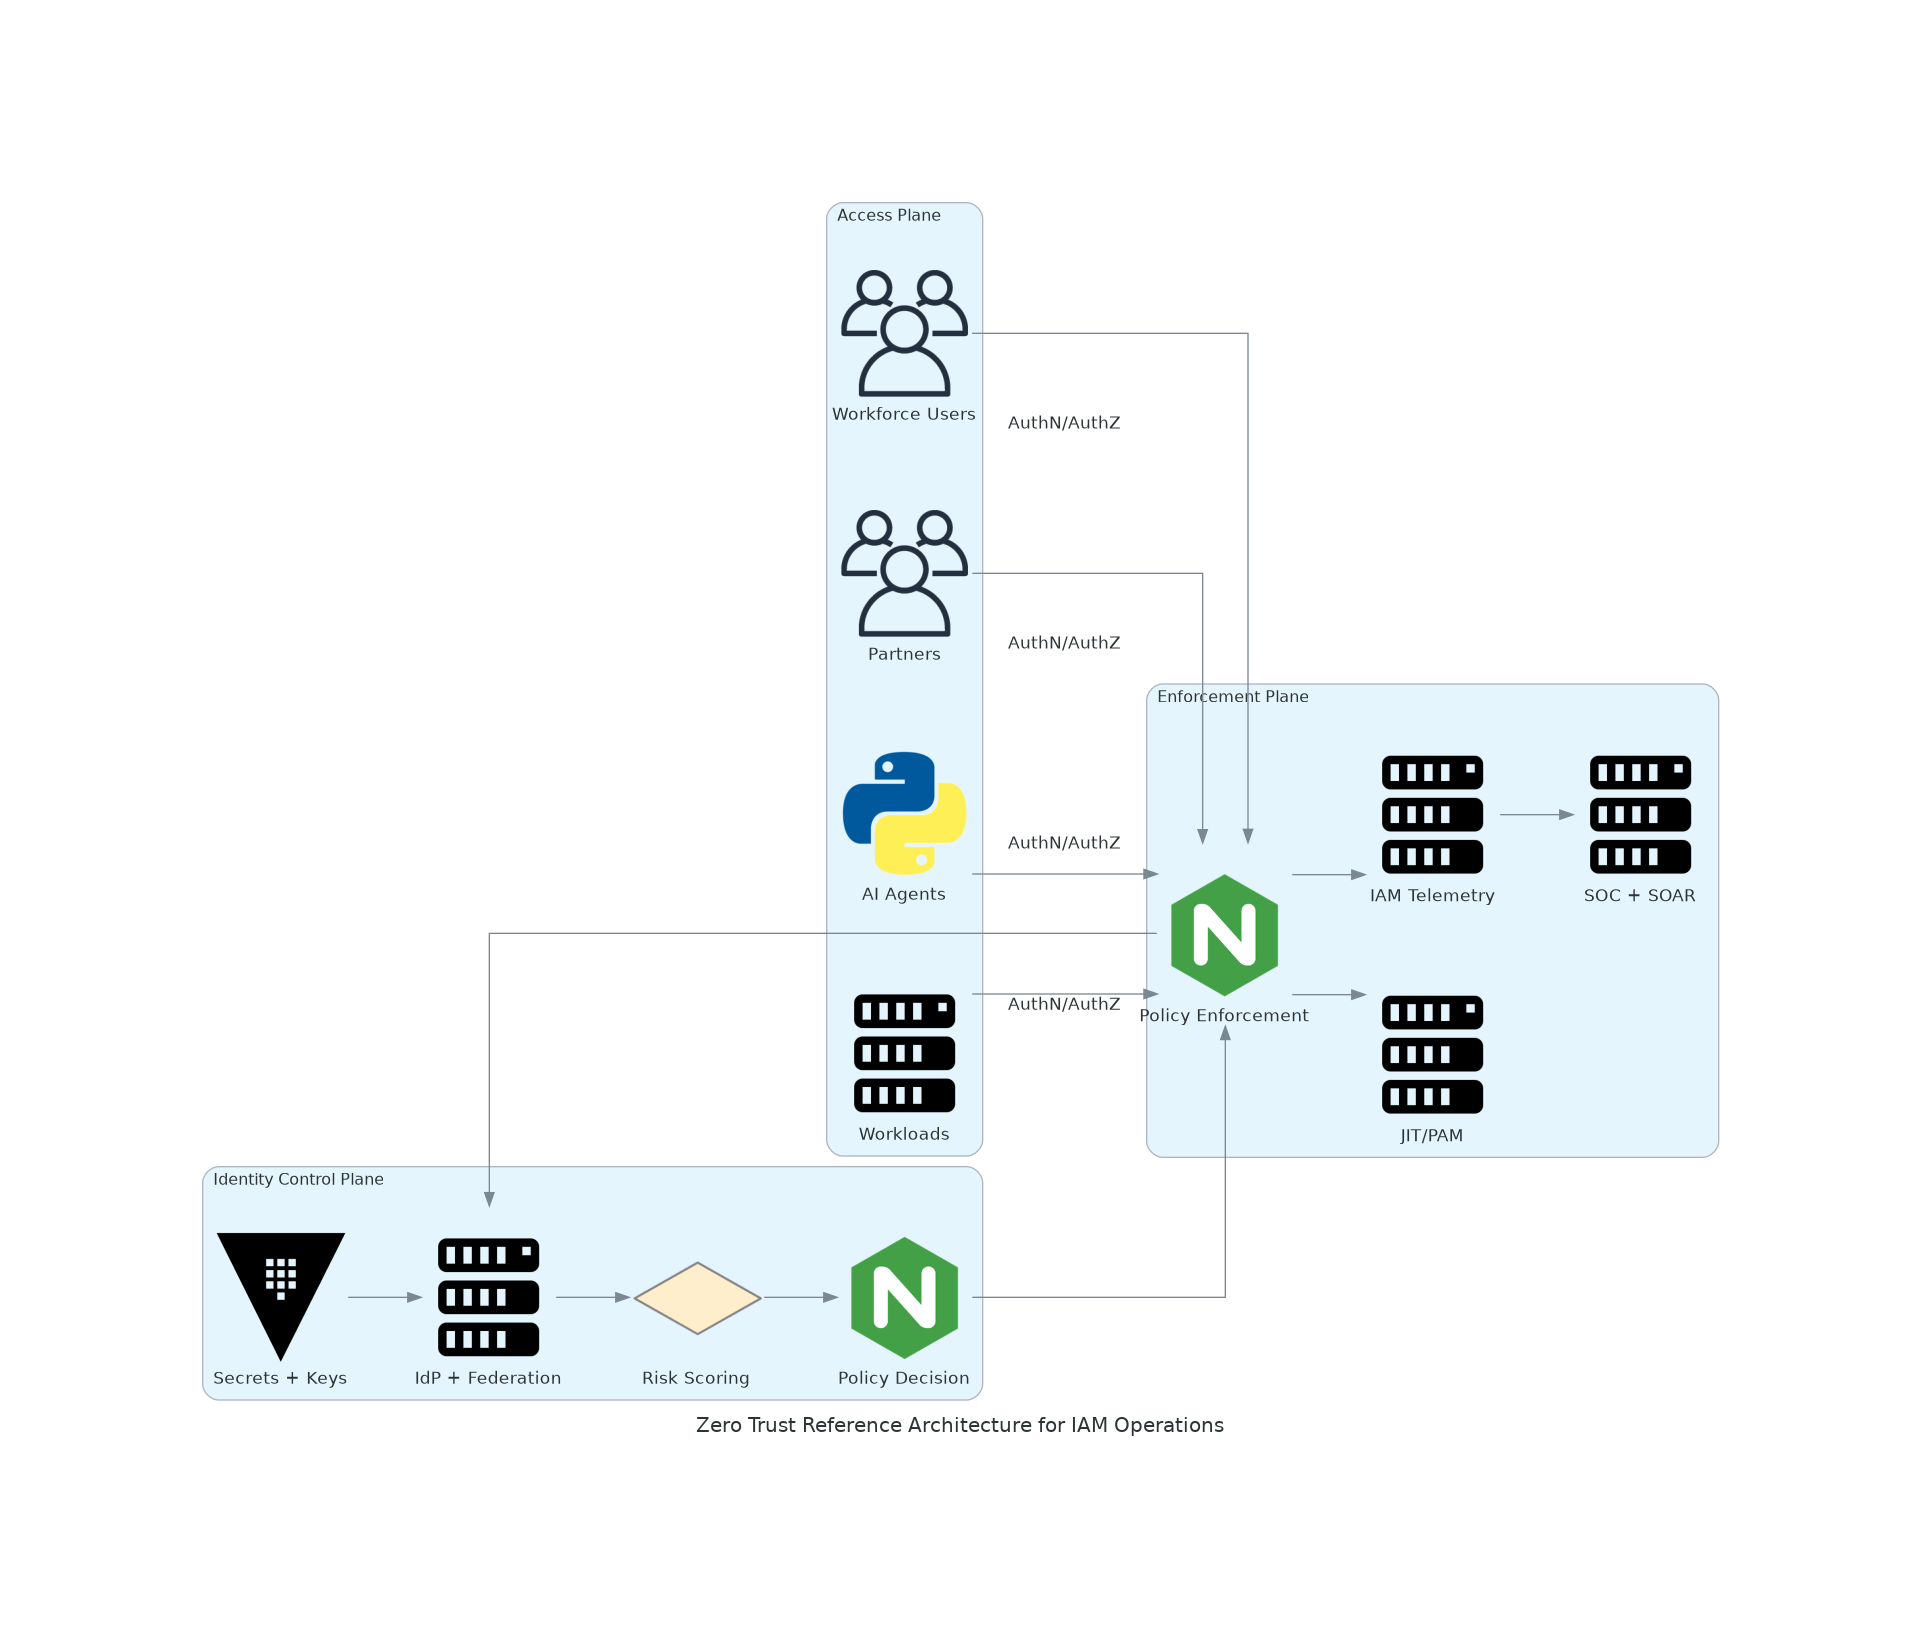
\includegraphics[width=0.98\textwidth]{figures/zero_trust_reference_architecture.png}
    \caption{Zero Trust IAM reference architecture for enterprise operations.}
    \label{fig:zta}
\end{figure}

\section{AI-Era Identity Risks and Mitigation Architecture}
\subsection{Agent Identity Lifecycle Controls}
Figure~\ref{fig:agentlife} models a lifecycle in which each AI agent is registered, attested, issued short-lived credentials, monitored continuously, and revocable in near real-time. This operational lifecycle aligns with NIST SP 800-63 assurance concepts for credential strength and session management, while extending them to autonomous machine actors \cite{nist_800_63}.

\begin{figure}[H]
    \centering
    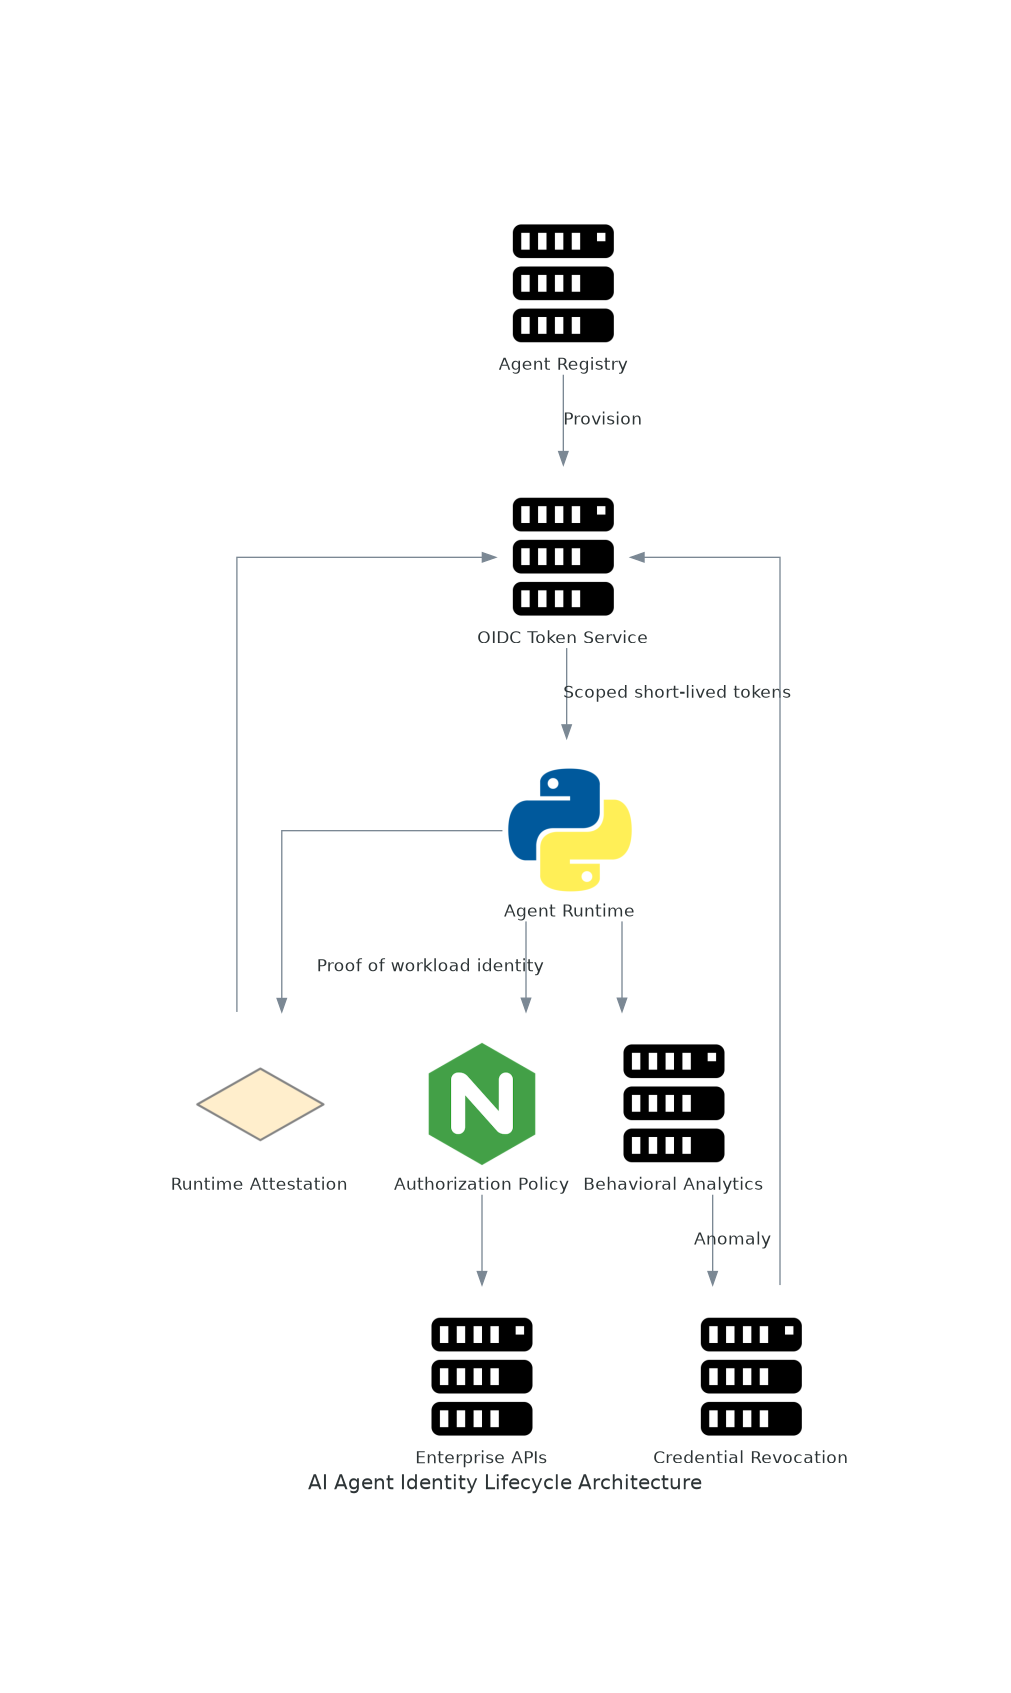
\includegraphics[width=0.86\textwidth]{figures/iam_ai_agent_lifecycle.png}
    \caption{AI-agent identity lifecycle architecture with attestation, token issuance, and revocation feedback loops.}
    \label{fig:agentlife}
\end{figure}

\subsection{Workload Identity and Secretless Patterns}
Operational policy should default to workload identity federation rather than static secrets. Key patterns include:
\begin{enumerate}[leftmargin=1.5em]
    \item Ephemeral credential issuance through federation (OIDC/JWT exchange) tied to runtime claims.
    \item Workload attestation checks before privileged token minting.
    \item Cryptographic key isolation and automated key rotation pipelines.
    \item Token binding and audience restriction to prevent replay in unintended services.
\end{enumerate}
These controls directly reduce CI/CD secret sprawl and decrease the dwell time of stolen credentials \cite{azure_workload_identity,aws_iam_roles_anywhere,slsa}.

\subsection{Just-in-Time Access and Continuous Verification}
Standing privileged roles are replaced with time-bounded elevation plus explicit approval and purpose metadata. Continuous verification should re-evaluate session trust on risk events such as impossible travel, unmanaged device use, suspicious API burst patterns, or anomalous agent behavior. This model is aligned with Zero Trust guidance that access decisions are dynamic and context-dependent \cite{nist_800_207,google_beyondcorp}.

\subsection{Device/User Risk Scoring and Behavioral Analytics}
High-value IAM operations require integrated user and entity behavior analytics (UEBA) with shared SOC/IAM ownership. Baselines should include geographic behavior, device integrity posture, API call sequence profiles, scope acquisition patterns, and token minting cadence. Detection outputs should drive immediate policy adaptation (step-up authentication, token narrowing, privileged action holds).

\subsection{Session Hardening and Phishing-Resistant MFA}
The operating standard for administrative and sensitive access should be phishing-resistant authenticators (FIDO2/WebAuthn, device-bound credentials) with strict re-authentication controls. This direction is consistent with federal Zero Trust mandates and modern identity assurance expectations \cite{executive_order_mfa,nist_800_63}. Session hardening requires:
\begin{itemize}[leftmargin=1.5em]
    \item short token lifetimes,
    \item refresh token rotation,
    \item token family revocation,
    \item impossible-travel and device-binding checks,
    \item explicit step-up for risky transaction classes.
\end{itemize}

\section{Incident-Driven IAM Architecture and Playbook Mapping}
\subsection{NIST-Aligned Operational Architecture}
To operationalize identity security, controls must map to incident lifecycle stages and measurable outcomes. NIST CSF 2.0 functions provide strategic framing \cite{nist_csf_2}; NIST SP 800-61r2 provides tactical incident flow \cite{nist_800_61}; NIST SP 800-207 and SP 800-63 provide identity and access architecture depth \cite{nist_800_207,nist_800_63}.

\begin{longtable}{>{\raggedright\arraybackslash}p{0.16\textwidth} >{\raggedright\arraybackslash}p{0.20\textwidth} >{\raggedright\arraybackslash}p{0.28\textwidth} >{\raggedright\arraybackslash}p{0.30\textwidth}}
\toprule
\textbf{NIST Function} & \textbf{IAM Objective} & \textbf{Operational Controls} & \textbf{SOC/IAM Runbook Mapping} \\
\midrule
\endhead
Govern & Define identity risk ownership and policy authority & IAM control charter, service ownership, exception governance, policy-as-code approvals & Weekly identity risk council; monthly exception burn-down; change freeze rules for critical auth services \\
Identify & Maintain visibility of identity assets and trust paths & Identity inventory, service account catalog, token issuer inventory, federation dependency map & Asset drift alerting; onboarding playbook for new SaaS/OIDC apps; identity dependency health checks \\
Protect & Enforce least privilege and resilient authentication & JIT elevation, phishing-resistant MFA, workload federation, conditional access & Privilege grant playbook with approvals; emergency break-glass controls; hardening baseline checks \\
Detect & Detect abuse of tokens, sessions, and privileged grants & UEBA detections, impossible travel, token replay analytics, OAuth scope anomaly rules & Severity-tiered detection use-cases, triage matrix, analyst enrichment query packs \\
Respond & Contain and eradicate identity incidents rapidly & Token family revocation, session kill, key rotation, federated trust disablement & Incident commander workflow; automated containment workflow; business communication templates \\
Recover & Safely restore identity-dependent services & staged access restoration, policy rollback controls, post-incident lessons learned & Recovery validation checklist; follow-up control tests; tabletop update and training plan \\
\bottomrule
\end{longtable}

\subsection{Incident Handling Lifecycle for IAM (SP 800-61r2)}
Figure~\ref{fig:irplaybook} presents an event flow aligned to SP 800-61r2 preparation, detection/analysis, containment/eradication/recovery, and post-incident activity. The design emphasizes evidence packaging, blast-radius assessment, controlled containment authority, and measurable recovery criteria.

\begin{figure}[H]
    \centering
    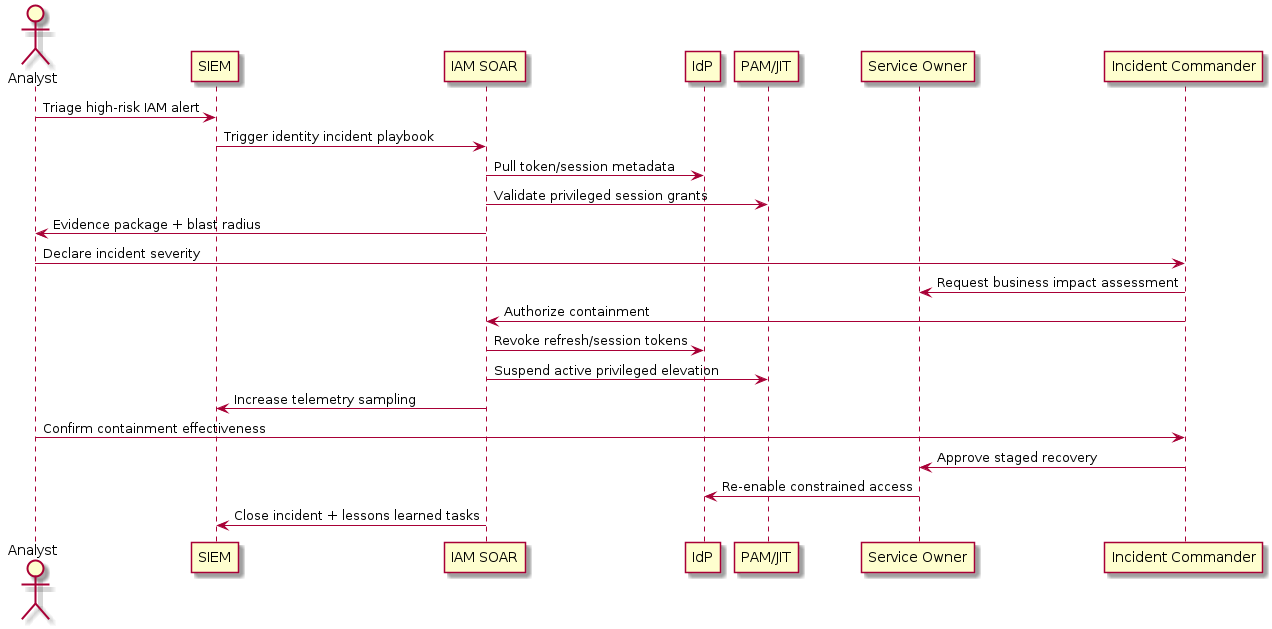
\includegraphics[width=0.92\textwidth]{figures/incident_response_playbook_flow.png}
    \caption{Incident response playbook sequence for high-risk IAM events.}
    \label{fig:irplaybook}
\end{figure}

\subsection{Detection Engineering Operating Pipeline}
\begin{figure}[H]
    \centering
    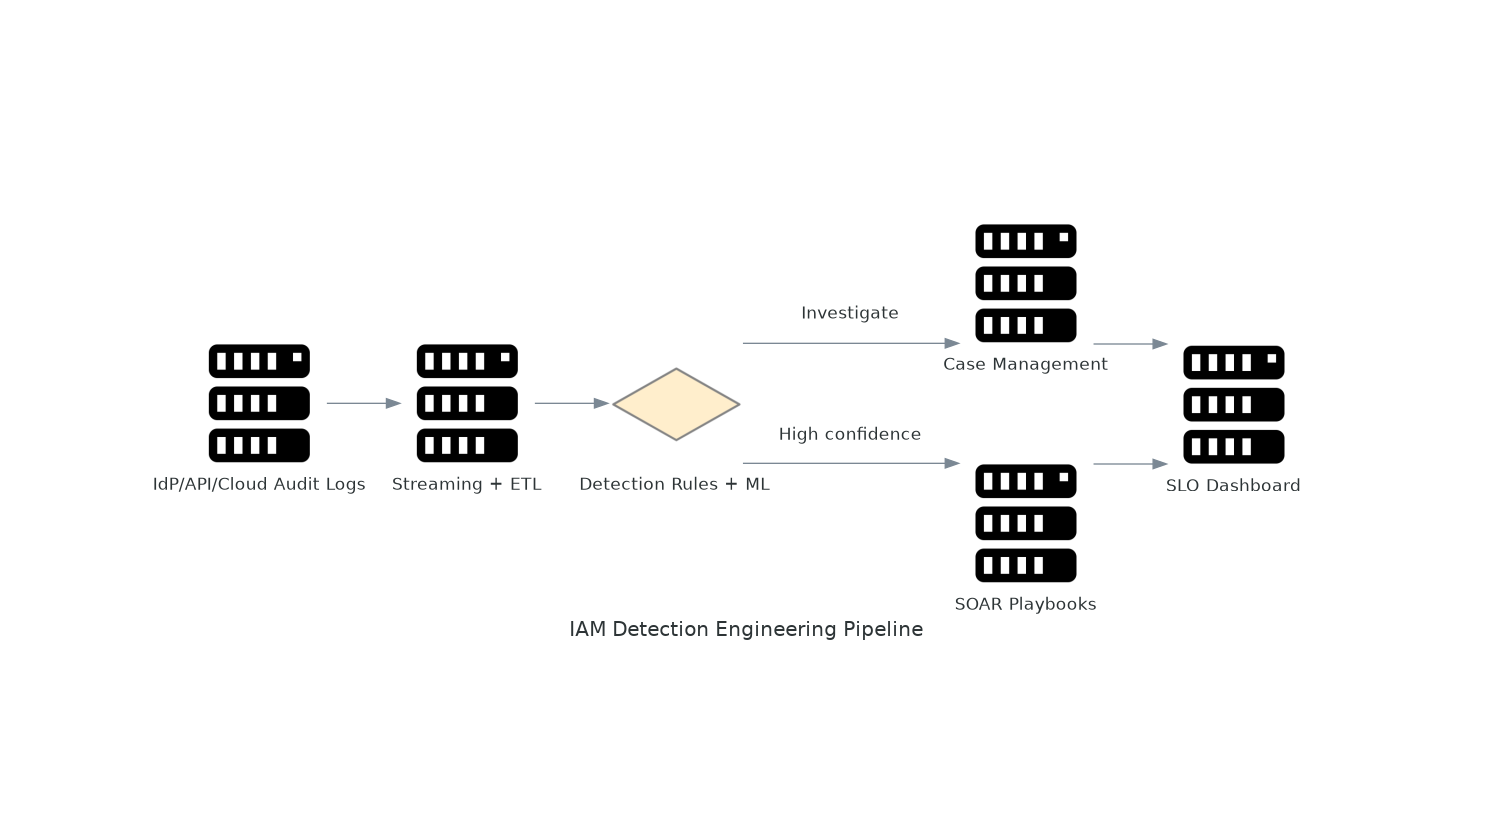
\includegraphics[width=0.94\textwidth]{figures/iam_detection_engineering_pipeline.png}
    \caption{Detection engineering pipeline connecting IAM telemetry to runbook automation and SLO reporting.}
\end{figure}

A production pipeline should include quality gates for detection precision, time-to-triage, and false-positive suppression. Detections are managed as code with controlled deployment, test datasets, and rollback plans. High-confidence detections trigger automatic containment actions; medium-confidence detections generate analyst-guided investigations.

\subsection{Token Compromise Response Sequence}
Figure~\ref{fig:tokenflow} models an adversary replaying a stolen token. The key architectural requirement is rapid movement from anomaly signal to token family revocation and forced re-authentication.

\begin{figure}[H]
    \centering
    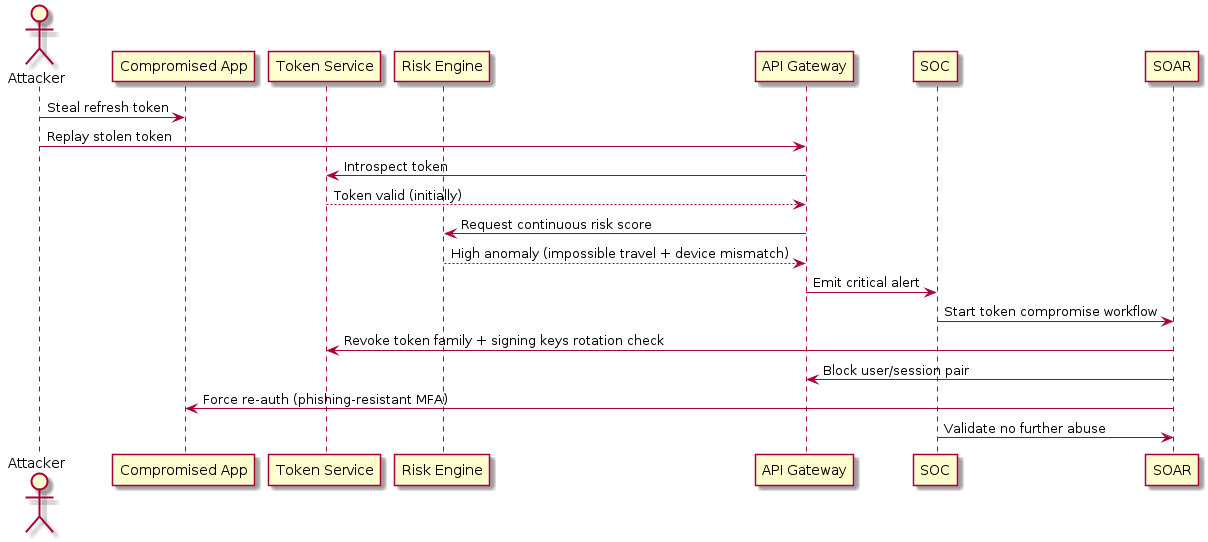
\includegraphics[width=0.90\textwidth]{figures/token_compromise_response_flow.png}
    \caption{Token compromise detection and automated containment flow.}
    \label{fig:tokenflow}
\end{figure}

\section{Real-World Incident Lessons Learned}
\subsection{Token Signing and Validation Failures}
The Microsoft Exchange Online intrusion reviewed by CSRB highlighted systemic risk from token-related trust weaknesses, key management controls, and monitoring gaps \cite{microsoft_storm0558,cisa_storm0558}. Core lessons include enforcing key isolation boundaries, improving token provenance telemetry, and hardening issuer validation logic for all resource providers.

\subsection{Identity Provider and Support-Channel Exposure}
The Okta support system compromise demonstrated that identity attack paths can originate in support and administrative workflows rather than only in production auth systems \cite{okta_support_breach}. This reinforces the need to apply identity assurance and strong session controls to all privileged support channels, including third-party support tooling.

SSO outages, configuration errors, and policy propagation failures also create significant business impact when identity services become single points of failure. Identity architecture must include graceful degradation controls, emergency access fallback processes, and predefined communication playbooks \cite{okta_status}.

\subsection{Supply-Chain Identity and CI/CD Credential Abuse}
Incidents involving CI/CD pipeline credential theft and package ecosystem compromise demonstrate that software delivery systems are identity systems in practice \cite{circleci_incident,slsa}. IAM programs must therefore include build identities, signing identities, and deployment identities under the same governance and detection regime used for workforce privileged access.

\subsection{Federation Trust Abuse and Cross-Cloud Risk}
Federation between enterprise identity and multiple cloud providers can produce privilege transitivity that is difficult to reason about. Figure~\ref{fig:crosscloud} illustrates a control model requiring explicit trust boundary documentation, issuer key integrity controls, and continuous verification for assumed roles.

\begin{figure}[H]
    \centering
    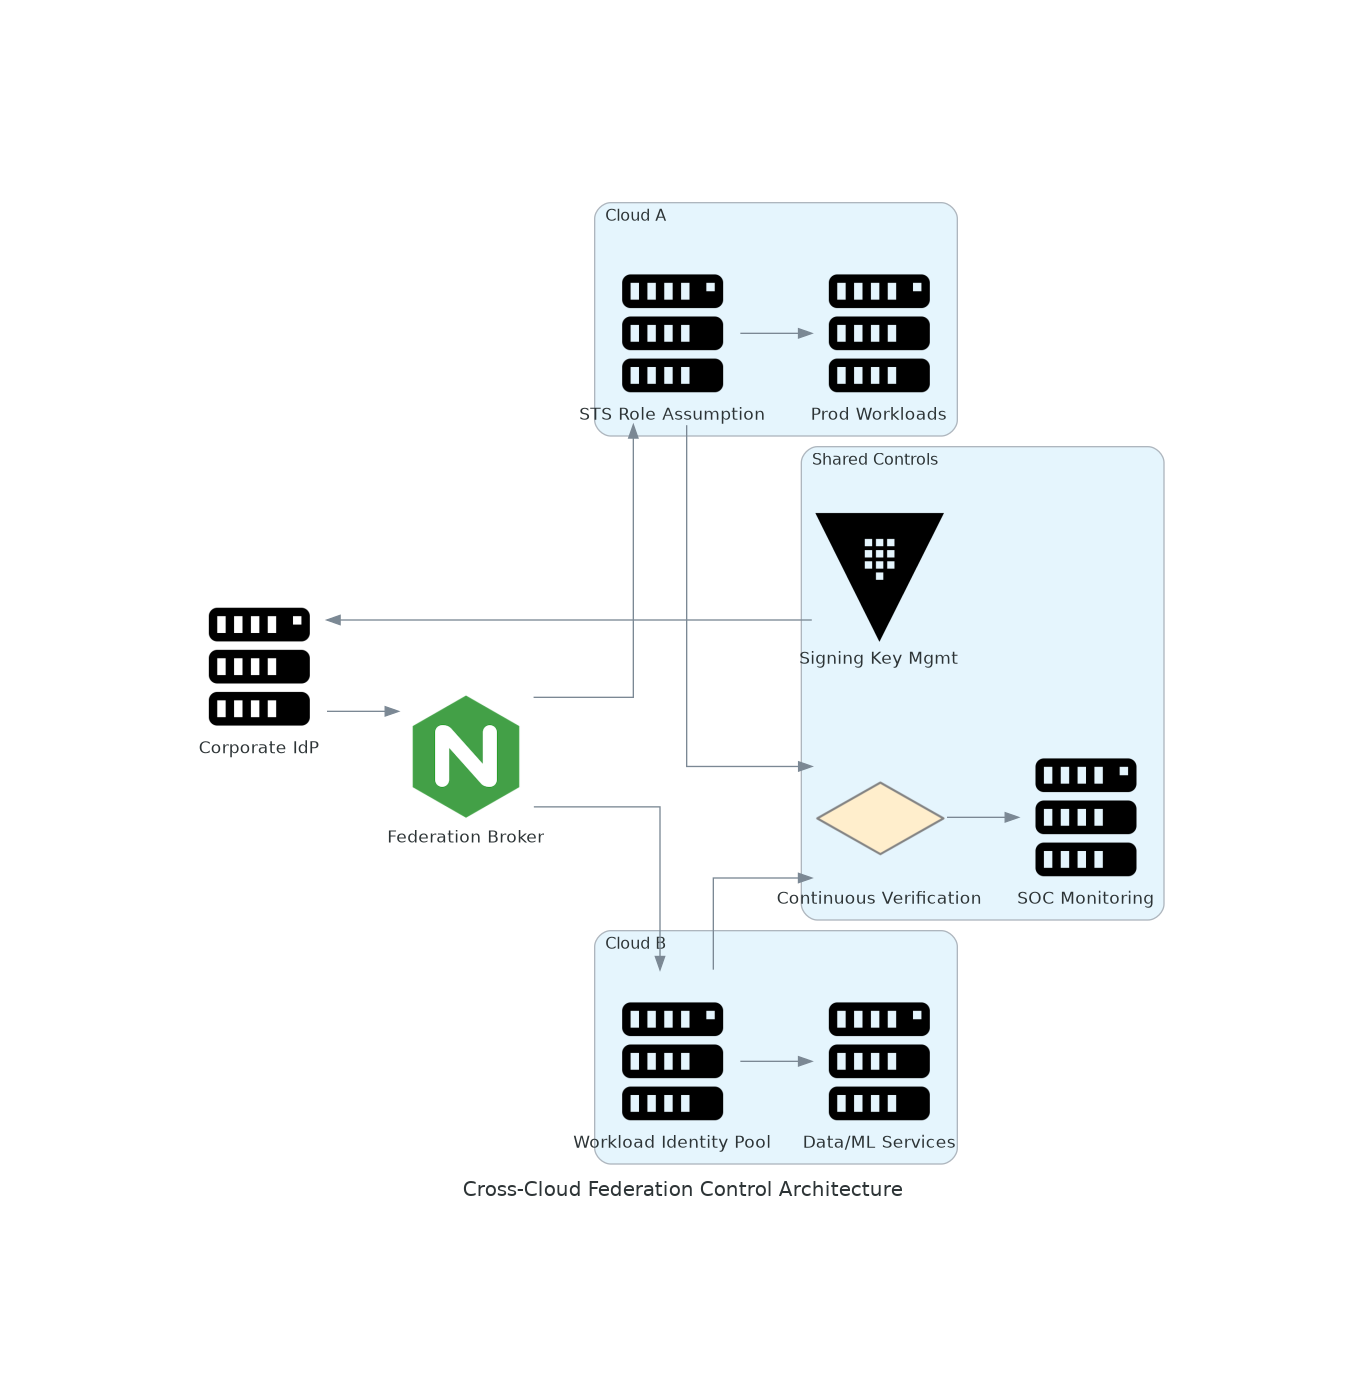
\includegraphics[width=0.96\textwidth]{figures/cross_cloud_federation_risk_controls.png}
    \caption{Cross-cloud federation architecture with shared control objectives and verification loops.}
    \label{fig:crosscloud}
\end{figure}

\section{Actionable IAM Operating Model for 2026}
\subsection{Reference Operating Model}
A resilient IAM operating model is built on four jointly governed layers:
\begin{enumerate}[leftmargin=1.5em]
    \item \textbf{Identity Services Layer}: IdP, federation broker, token service, credential lifecycle management.
    \item \textbf{Policy and Trust Layer}: conditional access, risk scoring, authorization policy engine, JIT controls.
    \item \textbf{Detection and Response Layer}: SOC pipelines, analytics, incident orchestration, containment automation.
    \item \textbf{Governance and Assurance Layer}: control objectives, KRIs/KPIs, audit evidence, tabletop and recovery testing.
\end{enumerate}

\subsection{Control Objectives}
\begin{itemize}[leftmargin=1.5em]
    \item \textbf{CO-1: Identity inventory completeness} for human and non-human identities with owner accountability.
    \item \textbf{CO-2: Authentication resilience} through phishing-resistant MFA and adaptive session controls.
    \item \textbf{CO-3: Privilege minimization} with JIT elevation and periodic privilege right-sizing.
    \item \textbf{CO-4: Token security} including short lifetimes, key rotation, issuer hardening, and revocation readiness.
    \item \textbf{CO-5: Detection coverage} mapped to ATT\&CK techniques relevant to identity abuse \cite{mitre_attck}.
    \item \textbf{CO-6: Incident readiness} with tested playbooks, authority model, and restoration checklists.
\end{itemize}

\subsection{Detection Engineering Use-Cases}
Table~\ref{tab:detections} lists practical SOC/IAM detections with expected action paths.

\begin{table}[H]
\centering
\small
\begin{tabular}{p{0.24\textwidth} p{0.24\textwidth} p{0.20\textwidth} p{0.24\textwidth}}
\toprule
\textbf{Use-Case} & \textbf{Signal Logic} & \textbf{Severity} & \textbf{Runbook Action} \\
\midrule
Impossible-travel privileged login & Same identity from geodistant regions within infeasible interval + admin role context & High & Suspend session, step-up challenge, analyst review \\
OAuth scope escalation & Sudden grant of high-risk scopes to low-baseline app/client & High & Revoke app grants, disable client, notify owner \\
Token replay anomaly & Repeated token use across divergent device fingerprints & Critical & Revoke token family, rotate keys if systemic, force re-auth \\
Service account misuse & Out-of-hours API burst from dormant workload identity & High & Disable workload principal, isolate workload, forensics \\
Federation drift & New trust relationship created outside change window & Medium/High & Auto-create incident, block trust propagation pending approval \\
MFA fatigue pattern & Multiple challenge denials followed by eventual approval & Medium & User outreach, risk score boost, conditional access hardening \\
\bottomrule
\end{tabular}
\caption{SOC/IAM detection engineering use-cases and response mapping.}
\label{tab:detections}
\end{table}

\subsection{Response SLAs and SLOs}
For identity-centric incident management, service-level definitions should be explicit and monitored continuously.
\begin{itemize}[leftmargin=1.5em]
    \item \textbf{SLA-R1: Detection-to-triage} under 15 minutes for critical token abuse alerts.
    \item \textbf{SLA-R2: Triage-to-containment} under 30 minutes for confirmed privileged compromise.
    \item \textbf{SLA-R3: Emergency revocation propagation} under 5 minutes across integrated services.
    \item \textbf{SLO-D1: Detection precision} above 85\% for high-severity identity detections.
    \item \textbf{SLO-D2: False-positive budget} below 10\% for automated containment triggers.
    \item \textbf{SLO-R1: Recovery confidence} 100\% completion of restoration checklist before closure.
\end{itemize}

\subsection{Tabletop Exercise Program}
Tabletop scenarios should be run quarterly with SOC, IAM engineering, platform operations, legal, and executive stakeholders. Minimum annual scenario set:
\begin{enumerate}[leftmargin=1.5em]
    \item IdP outage during peak business operations.
    \item Token signing key compromise with active replay.
    \item Federation trust abuse from partner tenant compromise.
    \item AI agent with over-privileged automation causing destructive changes.
\end{enumerate}
Each scenario should produce measurable outputs: decision latency, communication clarity, evidence quality, containment effectiveness, and recovery confidence.

\subsection{Maturity Roadmap}
\begin{longtable}{p{0.16\textwidth} p{0.26\textwidth} p{0.25\textwidth} p{0.25\textwidth}}
\toprule
\textbf{Phase} & \textbf{Primary Outcomes} & \textbf{Key Control Investments} & \textbf{Success Metrics} \\
\midrule
\endhead
0--6 months & Establish identity visibility and incident ownership & Identity inventory, privileged access baseline, incident role matrix, playbook minimum viable set & Inventory coverage $>$95\%, severity triage time baseline established \\
6--12 months & Reduce high-risk standing access and token risk & JIT/PAM rollout, workload federation migration, token telemetry normalization & Standing admin accounts reduced by 70\%, revocation SLA met consistently \\
12--18 months & Mature detection and automated containment & UEBA tuning, detection-as-code pipeline, SOAR runbooks for top attack paths & MTTD/MTTR improvements, lower false-positive rate, higher containment speed \\
18+ months & Continuous optimization and resilience validation & Cross-cloud trust verification, chaos testing for identity dependencies, advanced red-team scenarios & Reduced incident recurrence, improved business continuity, strong audit outcomes \\
\bottomrule
\end{longtable}

\section{Implementation Guidance and Governance Considerations}
\subsection{Program Governance}
Identity security outcomes require joint accountability across CISO leadership, identity engineering, SOC operations, and application/platform owners. Governance should explicitly define policy authority, emergency decision rights, and exception lifetimes. Identity architecture decisions that materially affect business continuity should be reviewed by enterprise risk governance functions, not only by engineering teams.

\subsection{Metrics and Reporting}
Executive reporting should include both risk and reliability dimensions:
\begin{itemize}[leftmargin=1.5em]
    \item privileged identity exposure trend,
    \item token misuse incident frequency,
    \item mean time to revoke and restore,
    \item percentage of critical applications with phishing-resistant MFA,
    \item percentage of non-human identities using short-lived federation credentials,
    \item number and age of policy exceptions.
\end{itemize}
Threat intelligence from industry reporting should inform quarterly control reprioritization \cite{verizon_dbir,crowdstrike_global_threat}.

\subsection{Design Principles to Sustain Over Time}
\begin{enumerate}[leftmargin=1.5em]
    \item Every identity action should be attributable to a principal, context, and approved policy path.
    \item Access should be continuously earned, not permanently granted.
    \item Detection and response controls are part of IAM architecture, not post-deployment add-ons.
    \item Identity resilience (availability + recoverability) is as important as identity confidentiality.
    \item Machine and agent identities must be governed with the same rigor as human privileged access.
\end{enumerate}

\section{Conclusion}
IAM operations architecture for 2026 must assume adversaries target identity infrastructure directly, exploit trust relationships across cloud and SaaS boundaries, and weaponize automation speed through compromised machine or agent credentials. A modern defense therefore combines identity assurance, Zero Trust policy execution, behavioral detection, and incident automation under a unified operating model.

The practical objective is not eliminating all identity incidents, but reducing blast radius and response time while preserving business continuity. By aligning architecture and runbooks to NIST CSF 2.0, SP 800-61r2, SP 800-63, and SP 800-207, organizations can move from static IAM controls to adaptive identity operations that remain effective under AI-era threat conditions.

\bibliographystyle{plain}
\bibliography{new-paper-references}

\end{document}
